\documentclass[tikz,border=5mm]{standalone}
\usepackage[T1]{fontenc}
\usepackage{fontspec}
\setmainfont{Fira Sans}[
  BoldFont=Fira Sans Bold,
  ItalicFont=Fira Sans Italic,
]
\usetikzlibrary{positioning, arrows.meta, shadows.blur, calc}

\definecolor{mTeal}{HTML}{2B7A78}
\definecolor{mBrown}{HTML}{C9956B}
\definecolor{mGray}{HTML}{888888}
\definecolor{mBg}{HTML}{FAFAFA}

\begin{document}
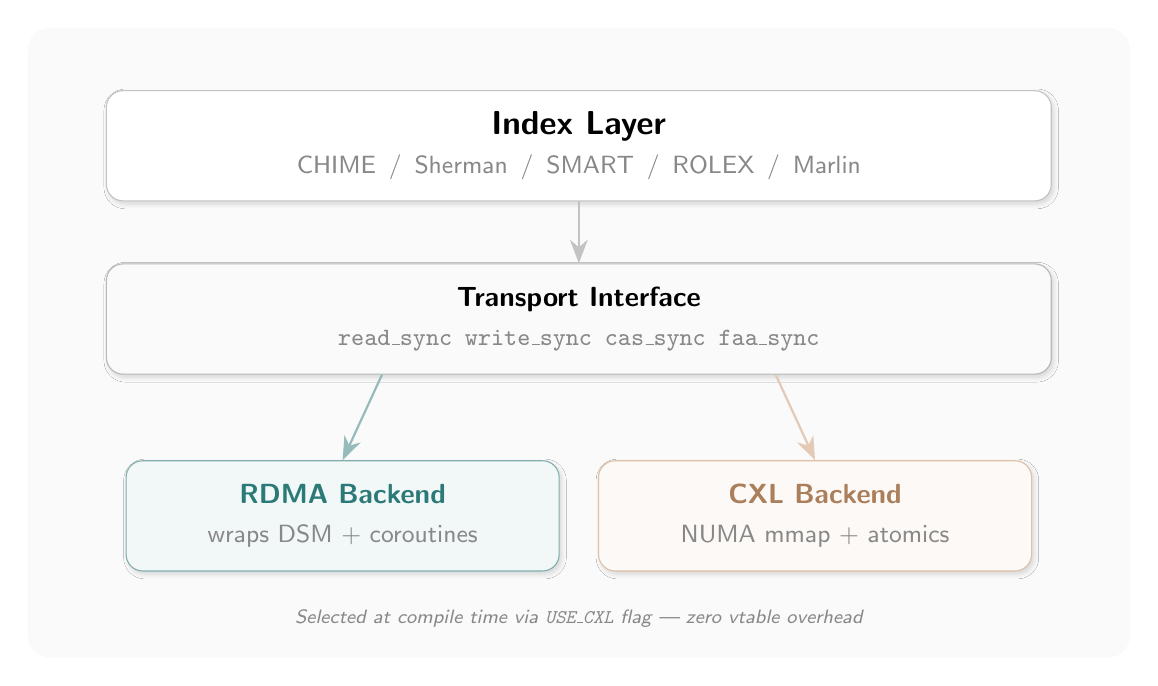
\begin{tikzpicture}[
  every node/.style={font=\sffamily},
  layer/.style={rounded corners=6pt, minimum height=1.4cm, align=center,
                blur shadow={shadow blur steps=6, shadow xshift=0.3mm,
                shadow yshift=-0.4mm, shadow opacity=15}},
  >=Stealth,
]
  \fill[mBg, rounded corners=8pt] (-7,-4) rectangle (7,4);

  % Index layer
  \node[layer, draw=mGray!50, fill=white, minimum width=12cm] (idx) at (0,2.5) {
    \textbf{\large Index Layer}\\[2pt]
    {\color{mGray}\small CHIME\enspace/\enspace Sherman\enspace/\enspace SMART\enspace/\enspace ROLEX\enspace/\enspace Marlin}
  };

  % Transport interface
  \node[layer, draw=mGray!60, fill=mGray!4, minimum width=12cm] (api) at (0,0.3) {
    \textbf{Transport Interface}\\[2pt]
    {\color{mGray}\small\texttt{read\_sync}\enspace\texttt{write\_sync}\enspace\texttt{cas\_sync}\enspace\texttt{faa\_sync}}
  };

  % RDMA backend
  \node[layer, draw=mTeal!60, fill=mTeal!6, minimum width=5.5cm] (rdma) at (-3,-2.2) {
    {\color{mTeal}\textbf{RDMA Backend}}\\[2pt]
    {\color{mGray}\small wraps DSM + coroutines}
  };

  % CXL backend
  \node[layer, draw=mBrown!60, fill=mBrown!6, minimum width=5.5cm] (cxl) at (3,-2.2) {
    {\color{mBrown!85!black}\textbf{CXL Backend}}\\[2pt]
    {\color{mGray}\small NUMA mmap + atomics}
  };

  % Arrows
  \draw[-{Stealth[length=3mm]}, thick, mGray!50] (idx.south) -- (api.north);
  \draw[-{Stealth[length=3mm]}, thick, mTeal!50] (api.south) ++(-2.5,0) -- (rdma.north);
  \draw[-{Stealth[length=3mm]}, thick, mBrown!50] (api.south) ++(2.5,0) -- (cxl.north);

  % Compile-time label
  \node[mGray, font=\sffamily\scriptsize\itshape] at (0,-3.5) {Selected at compile time via \texttt{USE\_CXL} flag --- zero vtable overhead};
\end{tikzpicture}
\end{document}
